%!TEX TS-program = XeLaTeX
\documentclass[11pt]{article}

\usepackage{amssymb}
\usepackage{amsthm}
\usepackage{amsmath}
\usepackage{mathtools}

\usepackage{fancyhdr}
\usepackage{graphicx}
\usepackage[top=3cm, left=2cm, right=2cm, headheight = 90pt]{geometry}
\usepackage{xltxtra}
\usepackage[font=small,labelfont=bf]{caption}

%%%%%%%%%%%%%%    Language matters  %%%%

%\usepackage[latvian]{babel}
%\usepackage[L7x]{fontenc}
%\usepackage[utf8x]{inputenc}

%%%%%%%%%%%%%%%%%%%%%%%%%%%%%%%%%%%7%%%%%

%%%%%%%%%%%%%%%%%%%%%%%%%%%       DO NOT EDIT         %%%%%%%%%%%%%%%%%%
%\usepackage{space}
%\renewcommand{\headrulewidth}{1pt}
%\fancyhead[L]{\includegraphics[width=3cm]{pictures/logo}}
%\fancyhead[R]{\raisebox{3ex}{\fbox{Language: \bf \lang}}}
\fancyhead[C]{{\Large\bf Pascals triangle - Problems}\\ \date}

\renewcommand{\theenumi}{\alph{enumi}}
%\newcommand{\problem}[1]{\paragraph{Problem #1.}}%<--------------- TRANSLATE THE WORD "Problem".
\fancyfoot[CE,CO]{}  % this is to remove page numbers (as you might want for single page docs)

\def\leq{\leqslant}
\def\geq{\geqslant}
\def\N{\mathbb N}
\def\R{\mathbb R}
\def\Z{\mathbb Z}
\DeclarePairedDelimiter\set\{\}
\newcommand{\?}{\stackrel{?}{=}}

%%%%%%%%%%%%%%%%%%%%%%%%%%%%%%%%%%%%%%%%%%%%%%%%%%%%%%%%%%%%%%%%%%%%%%%%%


%%% Language name in english %%%%%%%%%
\def\lang{Latvian}

%\def\lang{Lithuanian}

%%%%%%%%%%%%%%%%%%%%%%%%%%%%% TRANSLATE HERE %%%%%%%%%%%%%%%%%%%%%%%%%%%%%%%%%%

%\def\date{2018. gada 18. jūnijs}
%\def\notes{}


%%%%%%%%%%%%%%%%%%%%%%%%%%%%%%%%%%%%%%%%%%%%%%%%%%%%%%%%%%%%%%%%%%%%%%%%%%%%%%%

\def\prob{}

%%%%%%%%%%%%%%%%%%%%%%%%%%%%%%%%%%%%%%%%%%%%%%%%%%%%%%%%

\theoremstyle{definition}
\newtheorem{problem}{\prob}

\pagestyle{fancy}



\begin{document}
%\thispagestyle{fancy}
\noindent 
%\emph{\notes}

%1
\begin{problem}
\textit{[Formula of a triangle]}
Prove that $\binom{n}{r}+\binom{n}{r+1}=\binom{n+1}{r+1}$
\end{problem}
%

%2
\begin{problem}
\textit{[Construct of a triangle]} 
Construct a triangle from pointlike pins on a vertical plane so, that top row has one pin and each consequent row has one more pin than previous. A ball is dropped on a top pin so that, when it bounces off a pin, it has a equal chance to fall to left or right pin in next row downward (see Figure \ref{fig:pins}). 
\begin{center}
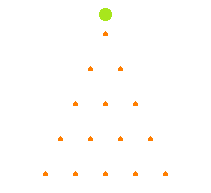
\includegraphics[width=2cm]{pins.png}
\captionof{figure}{Ball and triangle of pins }
\label{fig:pins}
\end{center}

Calculate the number of different paths that a ball can take to reach each pin! 
Is there any connection to result of problem \textit{[Formula of a triangle]}?

\end{problem}
%

%3
\begin{problem}
\textit{[Any number]} 
Does Pascals triangle contain number 2018?
\end{problem}
%

%4
\begin{problem}
\textit{[Powers of mystery]} 
By what factor the sum of elements of $101st$ row of Pascals triangle is greater than sum of elements of $100th$ row?
\end{problem}
%

%5
\begin{problem}
\textit{[Combinatorial proofs]} 
Prove combinatorically:
\begin{enumerate}
\item $\binom{2n}{2}=2\binom{n}{2} + n^2$
\item $\binom{2n+2}{n+1}=\binom{2n}{n+1} + 2\binom{2n}{n} + \binom{2n}{n-1}$
\end{enumerate}
\end{problem}
%

%6
\begin{problem}
\textit{[Binomial theorem]} 
Prove the \textit{Binomial Theorem}:
$$
(x+y)^n = \binom{n}{0}x^n+\binom{n}{1}x^{n-1}y+\binom{n}{2}x^{n-2}y^2+ \dots + \binom{n}{n-1}xy^{n-1} +\binom{n}{n}y^n = \sum_{i=0}^{n}{\binom{n}{i}x^{n-i}y^{i}}
$$
\end{problem}
%

%7
\begin{problem}
\textit{[Some sums]} 
Calculate following sums:
\begin{enumerate}
\item $\binom{5}{0}+2\binom{5}{1}+2^2\binom{5}{2}+\dots+2^5\binom{5}{5}$
\item $\binom{n}{0}-\binom{n}{1}+\binom{n}{2}-\dots+(-1)^n\binom{n}{n}$
\item $\binom{n}{0}+\binom{n}{1}+\binom{n}{2}+\dots+\binom{n}{n}$
\end{enumerate}
\end{problem}
%

\end{document}
